\documentclass[10pt,a4paper,UTF8]{article}
\usepackage{zclorg}
\author{zcl.space}
\date{}
\title{卷积编码和Viterbi译码}
\hypersetup{
 pdfauthor={zcl.space},
 pdftitle={卷积编码和Viterbi译码},
 pdfkeywords={communication viterbi ECC},
 pdfsubject={本文描述卷积编码和viterbi译码原理。},
 pdfcreator={Emacs 25.0.50.1 (Org mode 8.3.2)}, 
 pdflang={English}}
\begin{document}

\maketitle
\tableofcontents



\section{引言}
\label{sec:orgheadline1}


1965年,Peter Elias发明卷积码。1967年,Andrew J. Viterbi(高通的创始人之一)发明了一种高效的译码算法:Viterbi算法。Viterbi译码器可能是当前应用最广泛的一种卷积译码器。2005年,G. David Forney在南加州大学的Viterbi Conference上提到:每秒,全世界的Viterbi译码器恢复的的二进制比特数是 \(10^{15}\)。今天,我们来看看viterbi译码器如何实现译码。

\section{编码}
\label{sec:orgheadline2}


译码之前,先看如何卷积编码。描述卷积编码器的方法有很多,按照每种描述,我们都可以实现卷积编码。以约束长度为3,码率为1/2,生成多项式为 \(g_{0} = [1\quad 1\quad 1],g_{1}=[1  \quad 0 \quad 1]\)的卷积码为例,图\ref{fig:orgparagraph1}左侧给出了移位寄存器电路图表示,图\ref{fig:orgparagraph1} 右侧的表格是左侧的等价描述,显然左侧的表示更直观,右侧的表述更具体。

\begin{figure}[htb]
\centering
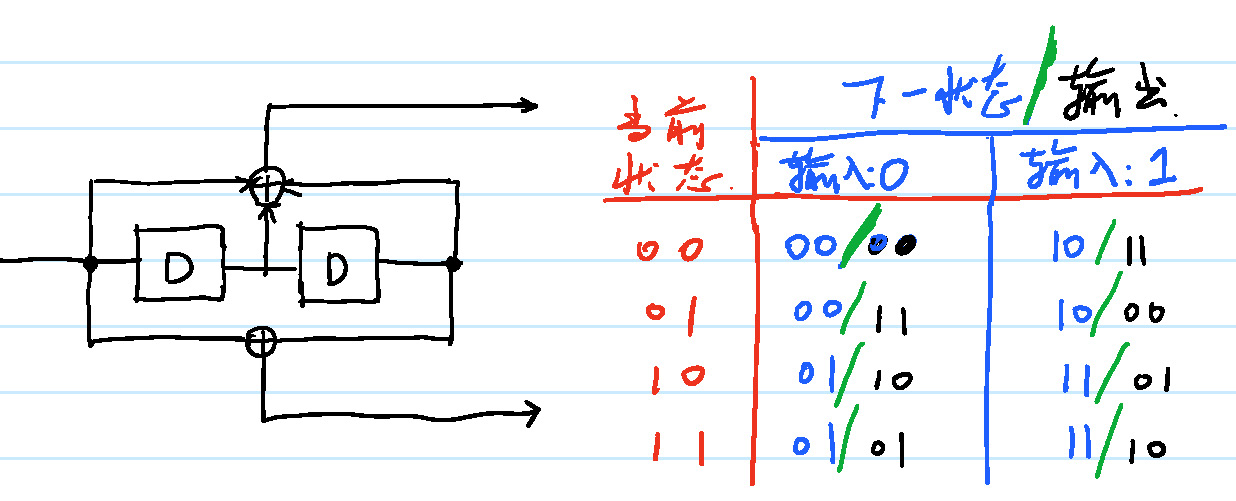
\includegraphics[width=0.6\textwidth]{../../img/20160101convolutionalEncoder.jpg}
\caption{\label{fig:orgparagraph1}
\textbf{卷积编码器的两种描述:移位寄存器和输入输出状态表}}
\end{figure}

卷积编码器还有一种描述:篱笆图描述。篱笆图让Viterbi译码过程生动了许多,我认为是一个很伟大的发明,其作用和法拉力用磁感线表示磁场的存在一样,让难以理解的抽象过程瞬间活灵活现。另外,在Turbo码的译码分析过程中,篱笆图也发挥着非常重要的作用。图\ref{fig:orgparagraph1}右侧的表格可以表示如图\ref{fig:orgparagraph2}所示。

\begin{figure}[htb]
\centering
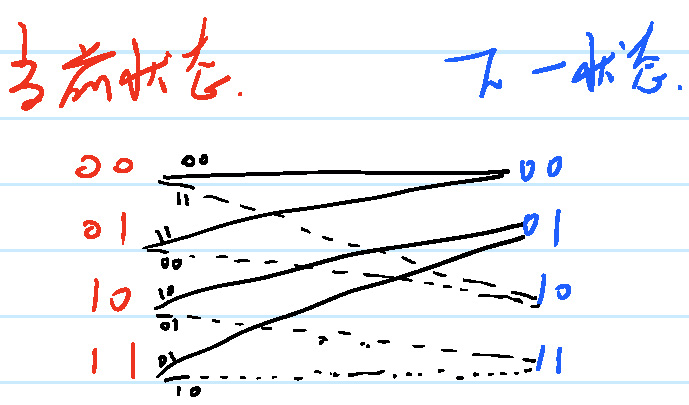
\includegraphics[width=0.6\textwidth]{../../img/20160101convolutionalEncoderTrellis.jpg}
\caption{\label{fig:orgparagraph2}
\textbf{卷积编码器篱笆图描述}}
\end{figure}


通过对篱笆图\ref{fig:orgparagraph2}进行时间上的延展,给定输入,我们可以很容易获得输出。假设输入为
\begin{equation}
\label{eq:1}
(010111001010001)_{2}
\end{equation}
则编码输出为
\begin{equation}
\label{eq:2}
(001110000110011111100010110011)_{2}
\end{equation}

输出的获得过程如图\ref{fig:orgparagraph3}所示。值得注意的是,在图\ref{fig:orgparagraph3}中, \(t=16\)和\(t=17\)时刻依然有0输入。这两个0的作用是冲洗编码器,使得编码器的状态归零。这样做的好处是Viterbi译码器知道编码器的最后一个状态是零状态。稍后我们会看到,Viterbi译码器译码有一个回溯的过程,如果知道编码器的最后一个状态是零状态,就避免了译码器瞎猜一个状态回溯,降低译码器的复杂度,尤其是减低了对内存的需求。稍后阐述译码过程时,我们会看到两个0的作用。在商用的通信协议中,比如3G和4G相关的协议,无论是采用Turbo码还是卷积码,都有译码器状态清零的操作。

\begin{figure}[htb]
\centering
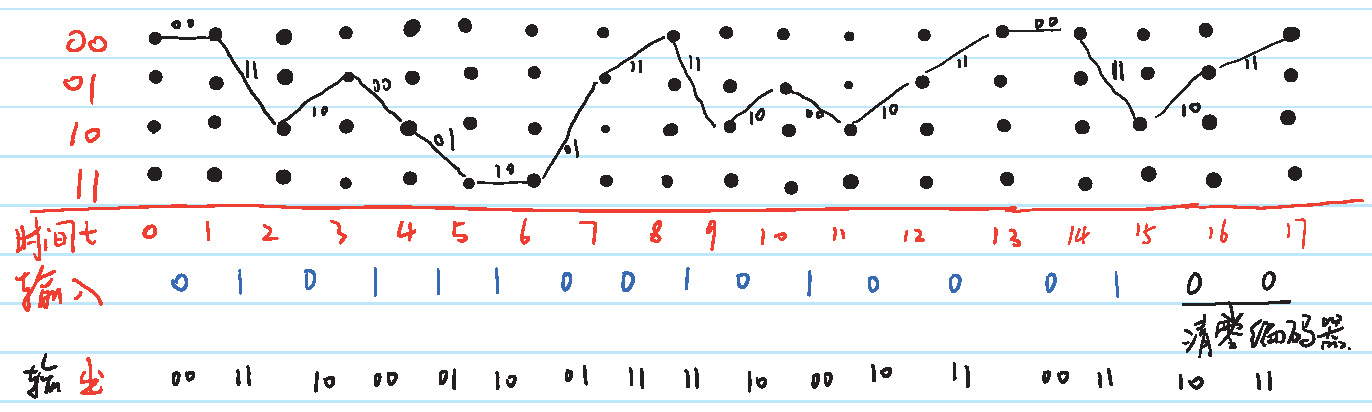
\includegraphics[width=0.6\textwidth]{../../img/20160101convolutionalEncoderTrellisOutput1.jpg}
\caption{\label{fig:orgparagraph3}
\textbf{针对输入序列利用篱笆图获得输出}}
\end{figure}

图\ref{fig:orgparagraph3}中的那条黑色路径就是编码器输入比特序列在编码器中留下的足迹。在图\ref{fig:orgparagraph3} 中,由于\(t=0\)时刻状态为00,从\(t=0\)到\(t=1\),只有两条路径可走:从00到00(输入为0);从00到10(输入为1)。从\(t=1\)到\(t=2\)有四条路径可走:从00和10出发各有两条路径。所以,在\(t,t>1\)时刻,编码器可能走过的路径有\(2^t\)。

Viterbi译码器译码就是根据收到的二进制比特,从最后一个状态回溯过程,找到最可能的哪条路径的过程。有点按图索骥的感觉。只不过由于信道的干扰,译码器不确定收到的序列是从哪条路径走过来生成的。所以译码器需要保留多条可能的路径,比较一番,选择最可能的那条路径。

接下来,我们就“按图索骥”,逐步演示Viterbi译码器的工作过程。每一个篱笆图都是我用onenote和Surface的触控笔做得。如果你之前没有这么一步一步的推演Viterbi译码过程,强烈建议你和我一样用纸和笔亲自画一遍。

\section{译码}
\label{sec:orgheadline3}


由于信道的不理想特性(比如衰落和噪声的存在),编码器输出到达接收端总是要经历一定程度的畸变,变得和发射的符号不一样。在图\ref{fig:orgparagraph4}中,接收符号在两个位置与发射比特不一致。

\begin{figure}[htb]
\centering
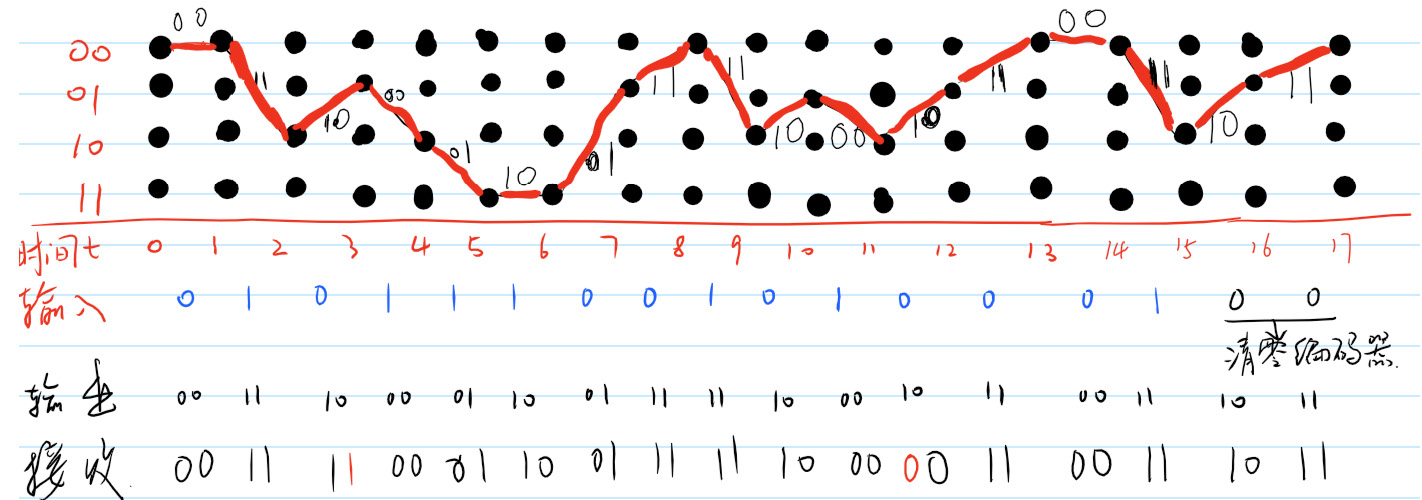
\includegraphics[width=0.6\textwidth]{../../img/20160101convolutionalReceiver.jpg}
\caption{\label{fig:orgparagraph4}
\textbf{信道的不确定性导致接收比特和编码器输出比特不一致}}
\end{figure}

每次我们收到一对经过信道的编码比特,都要与篱笆图上可能的状态转换输出的一对二进制比特比较,并计算汉明距离(就是看看有几个位置不一样)。显然,距离越近的就越像。

首先,当\(t=1\)时,接收到的符号为00。Viterbi译码器状态如图\ref{fig:orgparagraph5}所示。

\begin{figure}[htb]
\centering
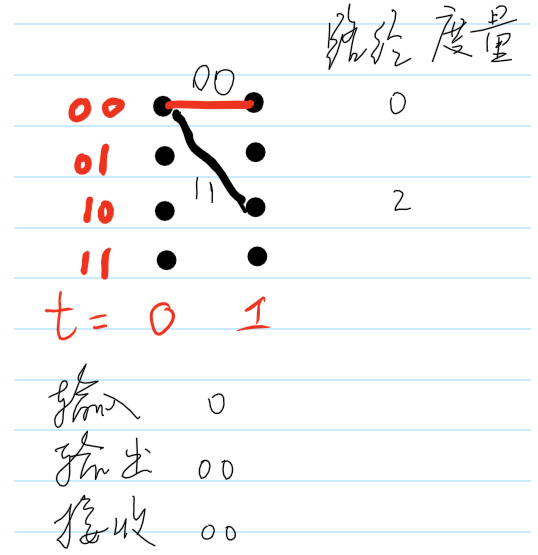
\includegraphics[width=0.6\textwidth]{../../img/20160101ViterbiT0.jpg}
\caption{\label{fig:orgparagraph5}
\textbf{\(t=1\)时的Viterbi译码器状态}}
\end{figure}

图\ref{fig:orgparagraph5}中,路径度量表示汉明距离的累积,由于目前只走了一步,所以汉明距离的累积就是这一步的汉明距离:分别是0和2。

当\(t=2\)时,接收到的符号为11。Viterbi译码器状态如图\ref{fig:orgparagraph6} 所示,图中用红色标示了最小路径度量的轨迹。另外\(t=2\)时,编码器的四个状态都有路径到达。从此以后,每个状态都有两个可能状态跳转而来。

\begin{figure}[htb]
\centering
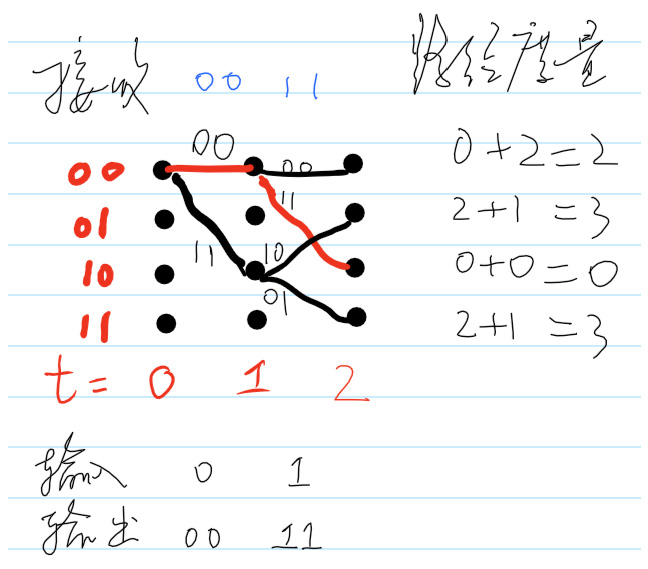
\includegraphics[width=0.6\textwidth]{../../img/20160101ViterbiT1.jpg}
\caption{\label{fig:orgparagraph6}
\textbf{\(t=2\)时的Viterbi译码器状态}}
\end{figure}

当\(t=3\)时,接收到的符号为11。如图\ref{fig:orgparagraph7}所示,每一个\(t=3\)时的状态都有两个\(t=2\)时的状态可以到达。所以\(t=3\)时需要比较八条路径的度量。此时路径上的输出太密,写不下,我把当前状态到下一状态的篱笆图附到右边便于查看。

\begin{figure}[htb]
\centering
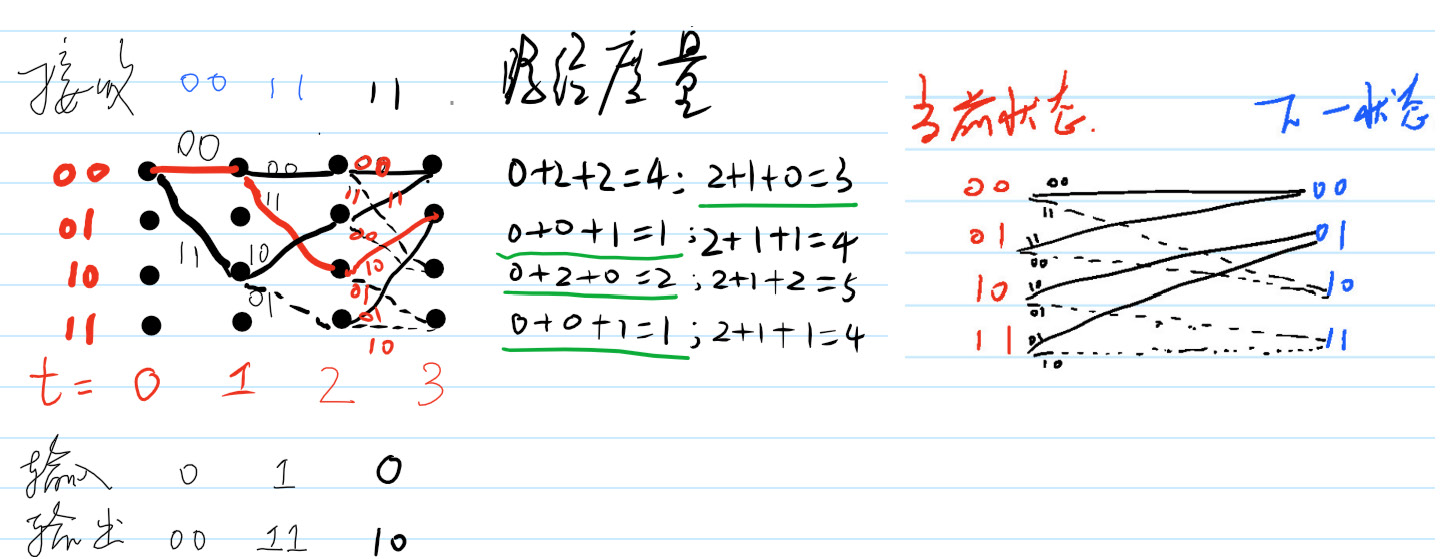
\includegraphics[width=0.6\textwidth]{../../img/20160101ViterbiT3.jpg}
\caption{\label{fig:orgparagraph7}
\textbf{\(t=3\)时的Viterbi译码器状态}}
\end{figure}

需要注意的是,第三对收到的二进制比特与发射的二进制比特有一个不同(发生了错误)。路径度量的计算结果中有两个最小的度量1,图\ref{fig:orgparagraph7}用红色标示了正确的路径,但是要记住还有一条路径的度量也是1。现在,接收机还不能判断收到的11是不是发射符号,即,译码器不确定从\(t=2\)到\(t=3\)发射端发射的是0还是1。只有当越来越多的二进制比特对到达译码器,译码器才能可靠的判断到底哪一条路径是正确的路径。

我们接着往下看。当\(t=4\)时Viterbi译码器的状态如图\ref{fig:orgparagraph8}所示。从图中可以看出只有一条路径的度量最小为1,该路径也是编码器编码过程中所使用的路径。此时我们可以看出\(t=3\) 时的接收符号错误已经得到了纠正。

\begin{figure}[htb]
\centering
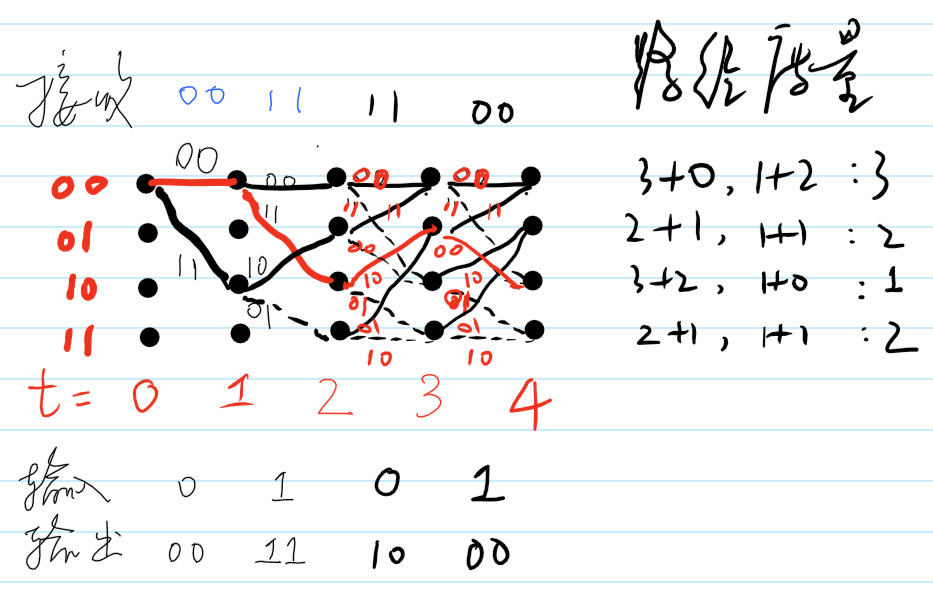
\includegraphics[width=0.6\textwidth]{../../img/20160101ViterbiT4.jpg}
\caption{\label{fig:orgparagraph8}
\textbf{\(t=4\)时的Viterbi译码器状态}}
\end{figure}

我们可以一直这么将篱笆图画下去,但是我不会这么做。我们直接来看看\(t=17\)时,接收机收到的篱笆图,如图所示。

\begin{figure}[htb]
\centering
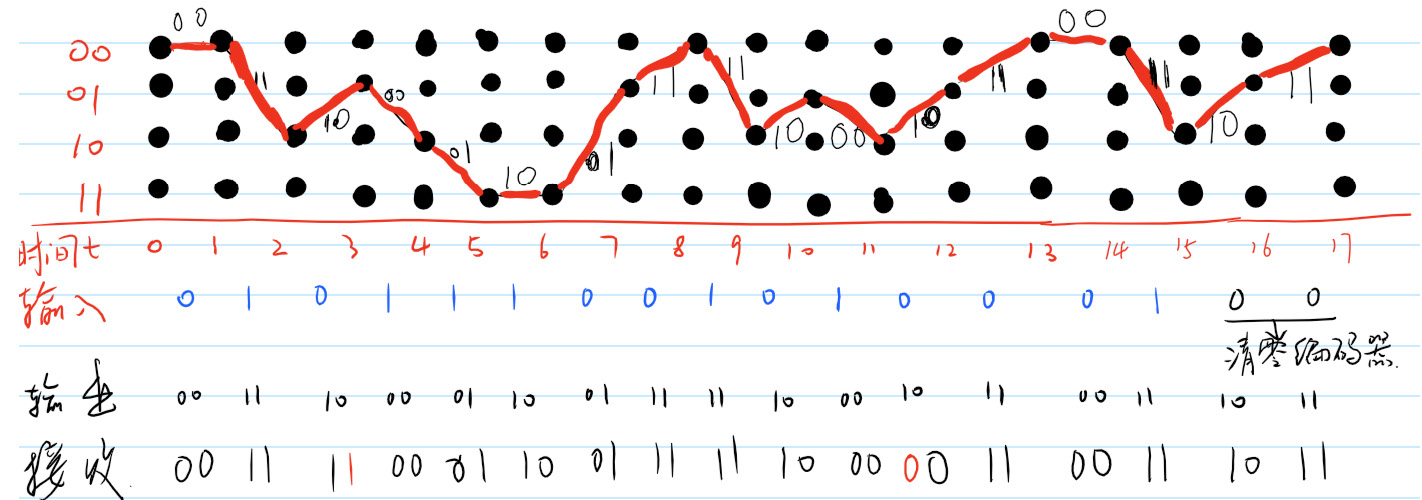
\includegraphics[width=0.6\textwidth]{../../img/20160101ViterbiT17.jpg}
\caption{\label{fig:orgparagraph9}
\textbf{\(t=17\)时的Viterbi译码器状态}}
\end{figure}

可以看出,图\ref{fig:orgparagraph9}和图\ref{fig:orgparagraph4}相同。这意味着Viterbi译码器找到了编码器走过的路,意味着接收符号序列中的两个错误没有对译码器正确译码造成影响,意味着译码器能克服信道对发送符号造成的这两次畸变。

当我们得到图\ref{fig:orgparagraph9}时,整个译码过程基本算是完成了,接下来我们要做的就是根据图\ref{fig:orgparagraph1}或者图\ref{fig:orgparagraph2}来找到最后这条路径上对应的输入比特即可。这个过程叫做回溯。
\section{回溯}
\label{sec:orgheadline4}


单独开一章讨论回溯过程。从图\ref{fig:orgparagraph5}到图\ref{fig:orgparagraph9}的过程中,每一次都记录了到达四个状态的l最小累计分支度量。对于本文给出的例子中一共记录了15个信息比特和2个清理比特对应的最小累计度量,这些最小累计分支度量如表\ref{tab:orgtable1}所示。

\begin{table}[htb]
\caption{\label{tab:orgtable1}
最小分支度量记录}
\centering
\begin{tabular}{lrrrrrrrrrrrrrrrrrr}
时间 & 0 & 1 & 2 & 3 & 4 & 5 & 6 & 7 & 8 & 9 & 10 & 11 & 12 & 13 & 14 & 15 & 16 & 17\\
\hline
状态00 &  & 0 & 2 & 3 & 3 & 3 & 3 & 4 & 1 & 3 & 4 & 3 & 3 & 2 & 2 & 4 & 5 & 2\\
状态01 &  &  & 3 & 1 & 2 & 2 & 3 & 1 & 4 & 4 & 1 & 4 & 2 & 3 & 4 & 4 & 2 & \\
状态10 &  & 2 & 0 & 2 & 1 & 3 & 3 & 4 & 3 & 1 & 4 & 1 & 4 & 3 & 3 & 2 &  & \\
状态11 &  &  & 3 & 1 & 2 & 1 & 1 & 3 & 4 & 4 & 3 & 4 & 2 & 3 & 4 & 4 &  & \\
\end{tabular}
\end{table}


有意思的是,在\(t=16\)和\(t=17\)时的最小累计度量和接收符号中错误比特的个数相同都是2. 从表\ref{tab:orgtable1}中我们知道了在\(t\)时刻,到达该状态的最小累计度量。我们还需要知道:在\(t\)时刻,到达该状态的前一个幸存状态是对少。比如在表\ref{tab:orgtable1}中,\(t=9\)时刻的状态10对应的最小分支度量是1,而\(t=9\)时刻的状态10是\(t=8\)时刻的状态00通过输入1跳转过来的,而不是状态01通过输入1跳转过来的。如果我们把表\ref{tab:orgtable1}中每一列中的最小值前后连起来,会发现,这条线和图\ref{fig:orgparagraph9}中的线几乎吻合。

为什么用“几乎”而不是“完全”? 从 \(t=17\)回溯到 \(t=13\)都很顺利,因为在表\ref{tab:orgtable1}中第13列到17列都只有一个最小分支度量,但是第12列却有两个最小分支度量2. 第13列的2是从12列的状态01对应的2跳转过来的还是从第12列的状态11跳转过来的呢?显然,结合编码器跳结构,我们知道只有从状态01才能一步跳转到状态00(通过输入0),从状态11无论如何一步也跳不到状态00. 同理从第4列跳转到第3列,第4列的最小度量1在状态10的位置,而第三列有两个最小分支度量1,分别位于状态01和状态11,我们知道只有状态01能一步跳转到状态10(通过输入1),而状态11无论如何也不能一步跳转到状态10.

\begin{table}[htb]
\caption{\label{tab:orgtable2}
最小分支度量幸存状态表}
\centering
\begin{tabular}{lrrrrrrrrrrrrrrrrrr}
时间 & 0 & 1 & 2 & 3 & 4 & 5 & 6 & 7 & 8 & 9 & 10 & 11 & 12 & 13 & 14 & 15 & 16 & 17\\
\hline
状态00 & 0 & 0 & 0 & 1 & 0 & 1 & 1 & 0 & 1 & 0 & 0 & 1 & 0 & 1 & 0 & 0 & 0 & 1\\
状态01 &  &  & 2 & 2 & 3 & 3 & 2 & 3 & 3 & 2 & 2 & 3 & 2 & 3 & 2 & 2 & 2 & \\
状态10 &  & 0 & 0 & 0 & 1 & 1 & 1 & 0 & 1 & 0 & 0 & 1 & 1 & 0 & 1 & 0 &  & \\
状态11 &  &  & 2 & 2 & 3 & 2 & 3 & 2 & 3 & 2 & 2 & 3 & 2 & 3 & 2 & 2 &  & \\
\end{tabular}
\end{table}

结合表\ref{tab:orgtable1} 和表\ref{tab:orgtable2} 我们可以得到图\ref{fig:orgparagraph9}中红线所示的幸存路径对应的前后状态转换,如表\ref{tab:orgtable3}所示。

\begin{table}[htb]
\caption{\label{tab:orgtable3}
幸存路径状态转换}
\centering
\begin{tabular}{lrrrrrrrrrrrrrrrrrr}
时间 & 0 & 1 & 2 & 3 & 4 & 5 & 6 & 7 & 8 & 9 & 10 & 11 & 12 & 13 & 14 & 15 & 16 & 17\\
\hline
 & 0 & 0 & 2 & 1 & 2 & 3 & 3 & 1 & 0 & 2 & 1 & 2 & 1 & 0 & 0 & 2 & 1 & 0\\
\end{tabular}
\end{table}

有了表\ref{tab:orgtable3},我们就可以顺藤摸瓜,沿着篱笆图把状态转换对应的输入比特找出来,这些输入比特就是译码输出序列。

可以看到,译码输出的信息比特序列为
\begin{equation}
\label{eq:3}
(01011100101000100)_{2}
\end{equation}

去掉两个尾比特,得到译码输出:
\begin{equation}
\label{eq:4}
(010111001010001)_{2}
\end{equation}

现在我们回顾一下Viterbi译码器工作的关键步骤。
\begin{enumerate}
\item 得到表\ref{tab:orgtable1} 。依赖篱笆图,我们可以使用纸和笔手动推演。
\item 记录跳转到当前状态的历史状态,即:得到表\ref{tab:orgtable2}。在生成表\ref{tab:orgtable1} 的过程中,顺带记录历史状态,即可得到表\ref{tab:orgtable2}。
\item 结合表\ref{tab:orgtable1} 和表\ref{tab:orgtable2} 以及编码器状态转移图\ref{fig:orgparagraph2},得到表\ref{tab:orgtable3} 。根据表\ref{tab:orgtable3}和图\ref{fig:orgparagraph2} 实现译码。
\end{enumerate}
\section{回溯深度}
\label{sec:orgheadline5}


在介绍译码过程中,我们把接收到的17对二进制比特全部送进译码器,计算累计路径度量,然后回溯,比较累计路径度量的大小,选择最小的那个路径。倘若输入译码器的二进制比特序列特别长,不是17对而是几千对,表\ref{tab:orgtable1}和表\ref{tab:orgtable2} 就会变得特别大。怎么办?截断。事实上,我们不需要等到把所有的接收符号都送入译码器计算累计路径度量,然后再回溯。实验表明,对于约束长度为 \(K\)的卷积码,回溯深度为 \(5K\)就不会带来性能损失。对于本文用到的例子,约束长度为3,每次我们只需要送入 \(5\times 3=15\)对二进制比特即可实现无性能损失的Viterbi译码。

\section{软译码}
\label{sec:orgheadline6}
\end{document}
